\section{Task 1}
\subsection{Step 1: Density Verification}

\begin{frame}{Analytic Hernquist}

	Density distribution:
	\begin{equation}
		\rho(r) = \frac{M}{2\pi}\frac{a}{r}\frac{1}{(r+a)^3}
		\label{eq:density-distribution}
	\end{equation}

	Cumulative Mass distribution inside a radius:
	\begin{equation}
		M(r) = M \frac{r^2}{(r+a)^2}
		\label{eq:cumulative-mass-distribution}
	\end{equation}

	Reformed Half-mass-radius equation, to get scale length
	\begin{equation}
		a = \frac{r_{1/2}}{1+\sqrt 2}
		\label{eq:scaling length}
	\end{equation}

	{\footnotesize Where:
	\begin{itemize}
		\item $M$  - Total mass of the system
		\item $a$ - Scale Length
		\item $r$ - Particle position vector
		\item $r_{1/2}$ - Half-mass radius: calculated numerically
	\end{itemize}}
\end{frame}

% since all particles have masses of 92. we assumed a mass of 1, to further simplify our equations
\begin{frame}{Numerical Density Approximation}
	Logarithmic binning of particles via \texttt{Histogram} class into a \texttt{std::vector} of \texttt{Shell}
	classes.
	\begin{equation}
		i_{log} = |\vb{r}|_{min} (\frac{|\vb{r}|_{max}}{|\vb{r}|_{min}})^{\frac {i_{lin}}{n}}
		\label{eq:lin-to-log}
	\end{equation}

	On histogram creation calculated for each shell:
	\begin{equation}
		\rho_i = M_i / V_i
		\label{eq:numeric-density}
	\end{equation}

	Poissonian density error with $\sigma = \sqrt{N / B}$:
	\begin{equation}
		\rho_{err} = \frac{\sigma}{V_i}
		\label{eq:density-error}
	\end{equation}

	{\footnotesize Where:
	\begin{itemize}
		\item $i$ - Shell index
		\item $B$ - Number of bins in histogram
		\item $N$ - Number of Particles
	\end{itemize}}

\end{frame}

\begin{frame}{Units}
	From assumption $G=1$ follows:

	\begin{itemize}
		\item $m$ - Mass per particle in Solar Masses (\si{\solarmass})
		\item $r$ - Position / length assumed as is, in Parsecs (\si{\parsec})
		\item $v$ - Velocity, assumed in \si{\kilo\metre\per\second} or \si{\parsec\per\year}
	\end{itemize}
\end{frame}

\begin{frame}
	\includegraphics[width=.95\textwidth]{figures/plots/hernquist.png}
\end{frame}

\subsection{Step 2: Direct Force Calculation}
\begin{frame}{Step 2: Analytic Force Reference}

	Taken from \cite{2008gady}, substituting $M(r)$ from Eq. (\ref{eq:cumulative-mass-distribution}) and
	reducing:
	\begin{equation}
		F(r) = - \frac{GM(r)}{r^2} \Rightarrow F(r) = - \frac{M}{(r+a)^2}
		\label{eq:newton-force}
	\end{equation}

	{\footnotesize Where:
	\begin{itemize}
		\item $M$ - Total Mass of System
		\item $r$ - Radius of shell
		\item $a$ - Scale length of System
	\end{itemize}}
\end{frame}

\begin{frame}{Step 2: Direct Force Calculation}
	\begin{equation}
		F_i=-G m_i \sum_{j=1}^N \frac{m_j}{\left[\left(\vb{r}_i-\vb{r}_j\right)^2+\varepsilon^2\right]^{3 /
				2}}\left(\vb{r}_i-\vb{r}_j\right)
		\label{eq:direct-force-full}
	\end{equation}

	% After applying assumptions
	% \begin{equation}
	% 	F_i = - \sum_{j=1}^N \frac{\left(\vb{r}_i-\vb{r}_j\right)}{\left[\left(\vb{r}_i-\vb{r}_j\right)^2+\varepsilon^2\right]^{3 /
	% 			2}}
	% 	\label{eq:direct-force-simple}
	% \end{equation}

	Taken from \cite{2008gady}, equation (2.227)
	\begin{equation}
		\epsilon=-\frac{r_{max}^2+\frac{3}{2} d^2}{\left(r_{max}^2+d^2\right)^{3 / 2}}
		\label{eq:softening}
	\end{equation}

	{\footnotesize Where:
	\begin{itemize}
		\item $i$ - Particle under consideration
		\item $\epsilon$ - Softening
		\item $r_{max}$ - Maximum radius
		\item $d$ - Mean inter-particle separation, calculated numerically once
		\item $G=1$
	\end{itemize} }
\end{frame}

\begin{frame}
	% \frametitle{Comparison}
	% With $O(N^2)$ computational complexity.\\

	\begin{figure}
		\centering
		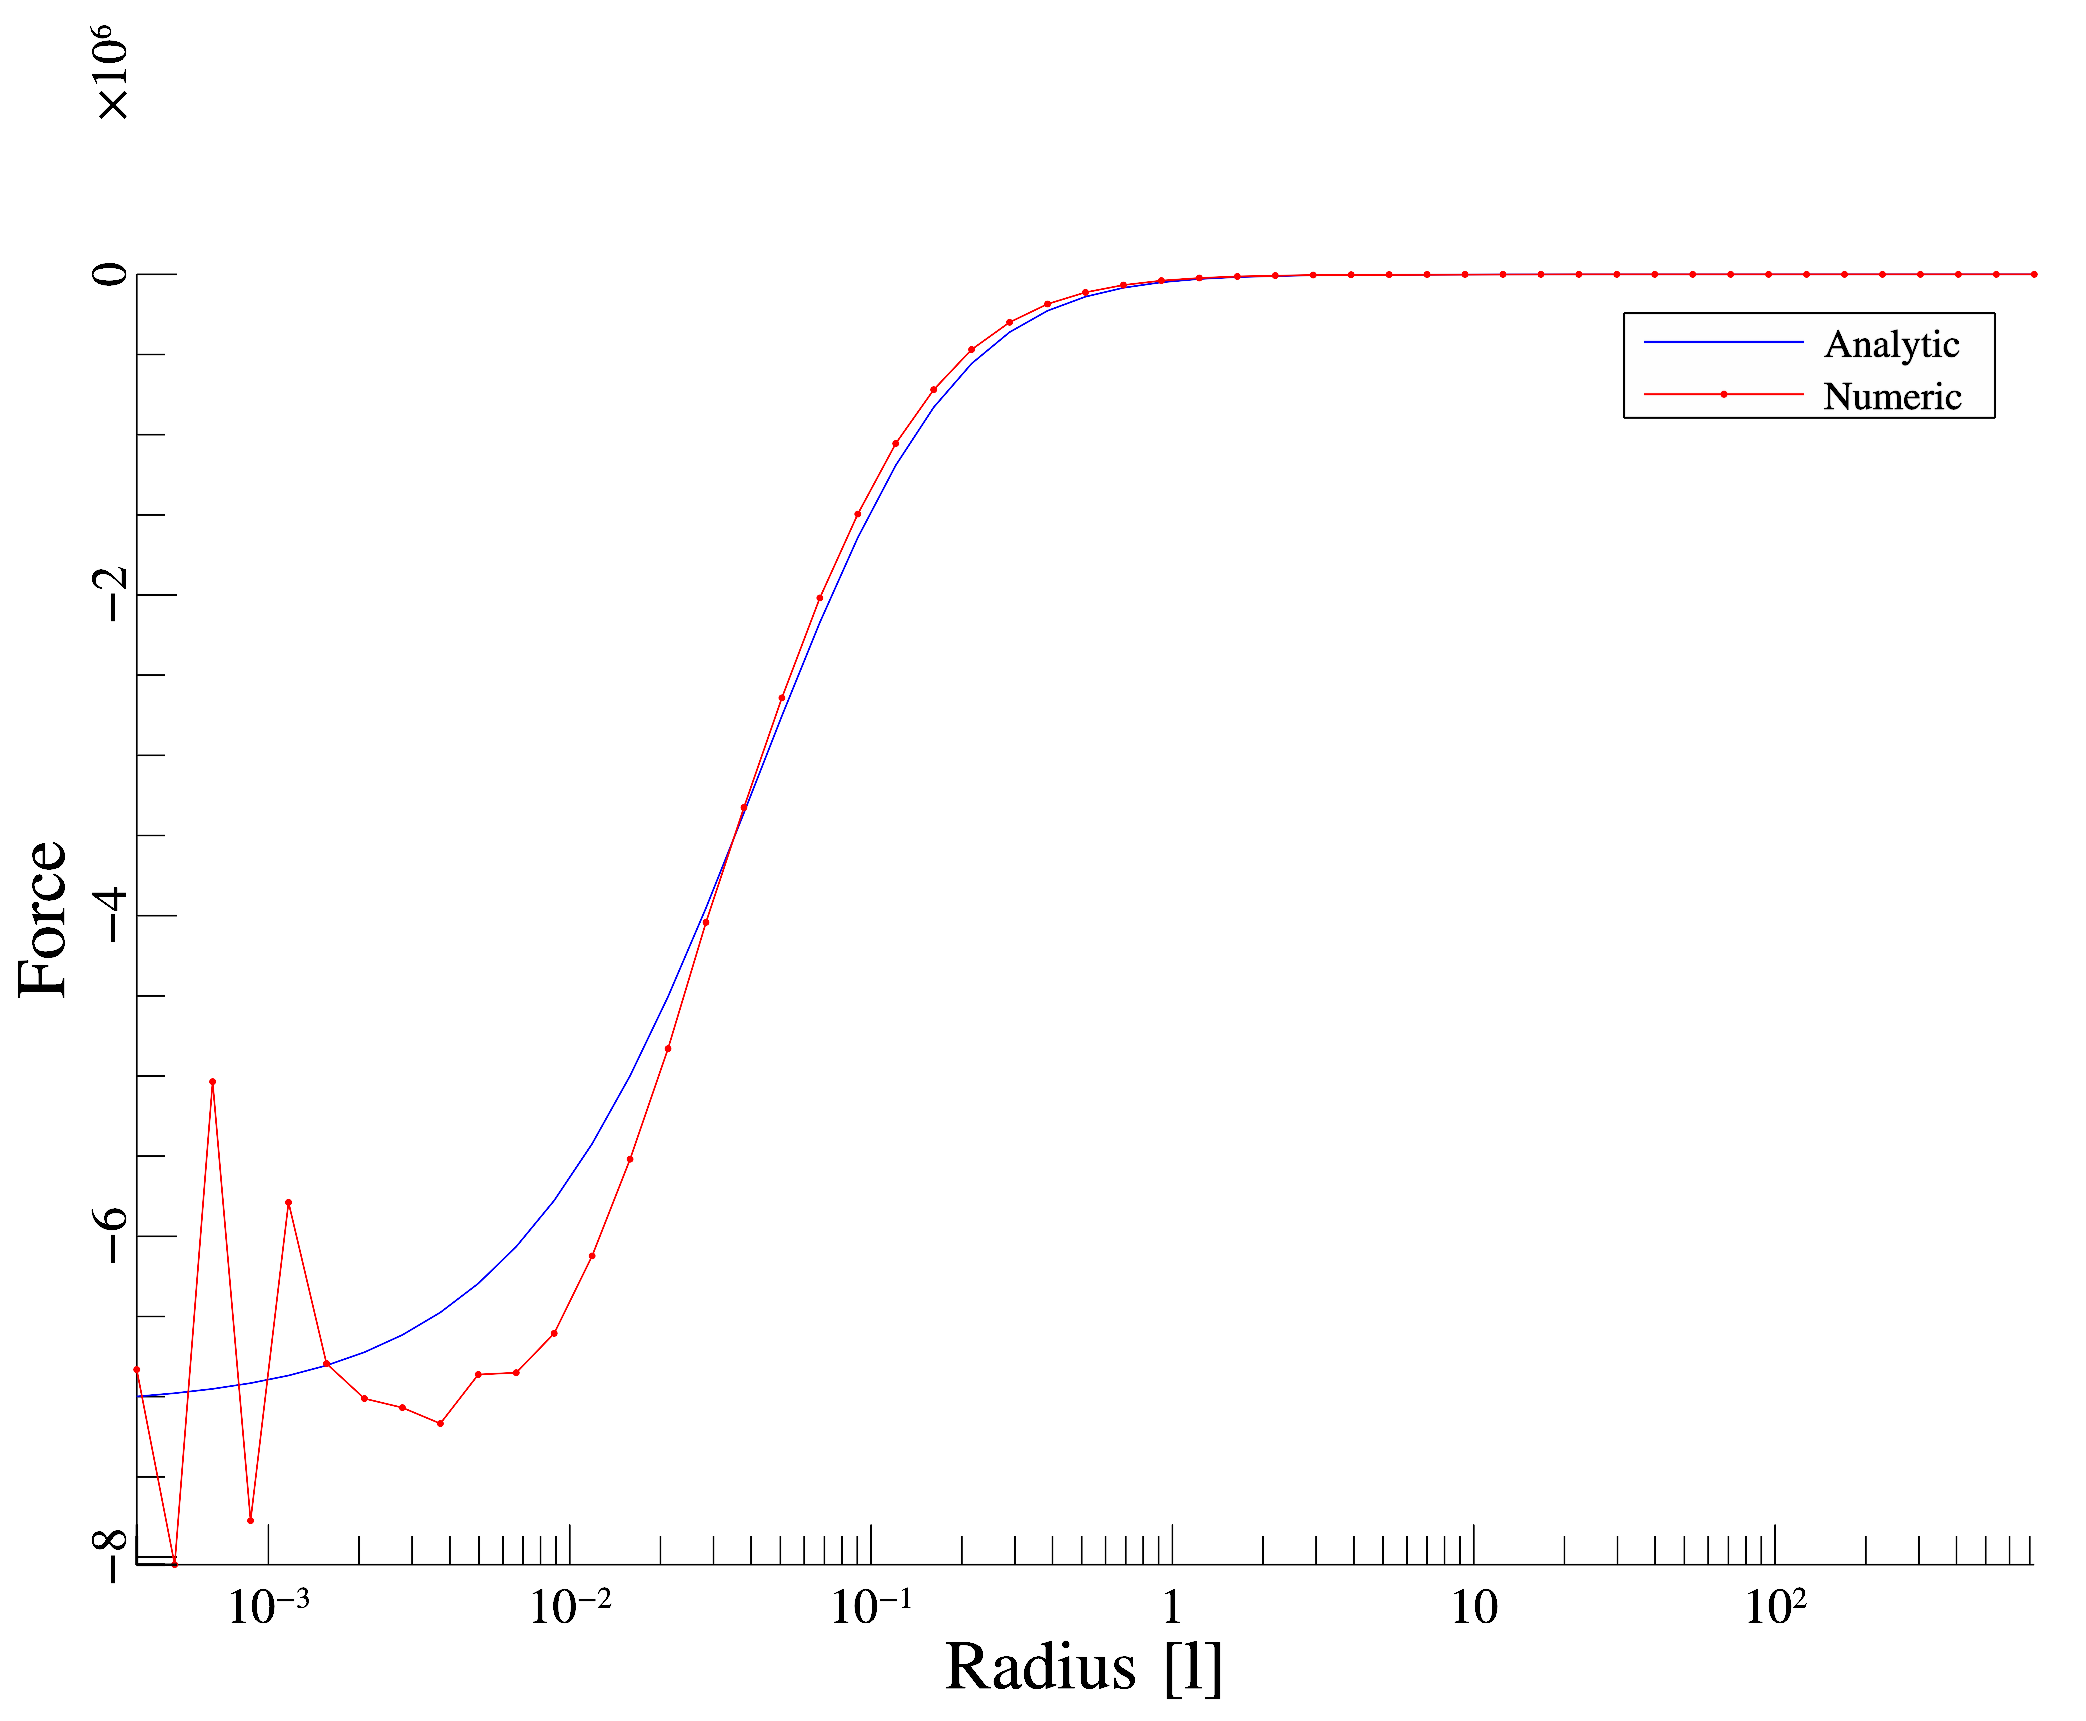
\includegraphics[width=0.95\textwidth]{figures/plots/forces.png}
		% \caption{}\label{fig:}
	\end{figure}

\end{frame}

\begin{frame}{Relaxation Timescale}
	% Increasing the gravitational softening above the interparticle separation alters the close encounters between particles.
	% It reduces the impact of these encounters on particle trajectories.
	% As a result, the energy exchange during encounters becomes less efficient. This would typically lead to an 
	% increase in the relaxation timescale, because it would take longer for the system to reach equilibrium due to
	% the less frequent and less effective energy exchanges.

	% Although, since the relaxation calculation is purely analytical, there is no real correlation between the
	% values.

	\begin{equation}
		v_c = \sqrt{GM(R_{hm})/R_{hm}}
		\label{eq:circular-velocity}
	\end{equation}
	\begin{equation}
		t_{cross} = \frac{R_{hm}}{v_c}
		\label{eq:crossing_timescale}
	\end{equation}
	\begin{equation}
		t_{relax} = \frac{N}{8\ln{N}}t_{cross}
		\label{eq:relaxation_timescale}
	\end{equation}

	\bigskip

	Using $G = \SI{4.3009172706e-3}{\parsec.\solarmass^{-1}.(\kilo\metre\per\second)^2}$ and $m = \SI{92.4259}{\solarmass}$: \\

	Crossing Timescale: $898.302\ yr$ \\
	Relaxation Timescale: $0.520\ Myr$

\end{frame}

